\documentclass[preview]{standalone}

\usepackage{amsmath}
\usepackage{amssymb}
\usepackage{tikz}
\usepackage{wrapfig}
\usepackage{xfrac}
\usepackage{bettelini}
\usepackage{stellar}
\usepackage{definitions}

\begin{document}

\id{measuretheory-simple-functions}
\genpage

\section{Simple functions}

\begin{snippetdefinition}{simple-function-definition}{Simple function}
    Let \(X\) be a \set. A \function \(s\colon X\fromto\complexnumbers\) is a
    \emph{simple function} if its image \(s(X)\) is finite. If \((X,\Sigma)\)
    is a \measurablespace and \(s\) is measurable, then \(s\) is called a
    \emph{measurable simple function}.
\end{snippetdefinition}

\begin{snippetproposition}{simple-function-measurable-fibres}{Measurability of a simple function}
    Let \((X,\Sigma)\) be a \measurablespace and let
    \(s\colon X\fromto\complexnumbers\) have finite image. Then \(s\) is
    measurable if and only if
    \[
        s^{-1}(\{\alpha\})\in\Sigma
        \qquad\text{for every }\alpha\in s(X).
    \]
\end{snippetproposition}

\begin{snippetproof}{simple-function-measurable-fibres-proof}{simple-function-measurable-fibres}{Measurability of a simple function}
    If \(s\) is measurable, every fibre is measurable because singletons are
    Borel. Conversely, for every Borel set \(B\subseteq\complexnumbers\),
    \[
        s^{-1}(B)
        =\bigcup_{\alpha\in B\intersection s(X)}s^{-1}(\{\alpha\}).
    \]
    This is a finite union of measurable fibres.
\end{snippetproof}

\begin{snippetproposition}{simple-function-indicator-representation}{Indicator representation of a simple function}
    Let \(s\colon X\fromto\complexnumbers\) be a \simplefunction with
    \(s(X)=\{\alpha_1,\ldots,\alpha_m\}\), and set
    \(A_i=s^{-1}(\{\alpha_i\})\). Then the sets \(A_i\) form a partition of
    \(X\), and
    \[
        s=\sum_{i=1}^m\alpha_i\indicator_{A_i}.
    \]
    If \((X,\Sigma)\) is measurable, then \(s\) is measurable exactly when
    every \(A_i\) belongs to \(\Sigma\).
\end{snippetproposition}

\section{Approximation by simple functions}

\begin{snippettheorem}{nonnegative-measurable-simple-approximation-theorem}{Approximation by nonnegative simple functions}
    Let \((X,\Sigma)\) be a \measurablespace and let
    \(f\colon X\fromto[0,+\infty]\) be measurable. There exists a sequence of
    nonnegative measurable simple functions \(s_n\) such that
    \[
        s_n(x)\uparrow f(x)
        \qquad\text{for every }x\in X.
    \]
    The sequence can be chosen to converge uniformly if and only if \(f\) is
    bounded.
\end{snippettheorem}

\begin{snippetproof}{nonnegative-measurable-simple-approximation-theorem-proof}{nonnegative-measurable-simple-approximation-theorem}{Approximation by nonnegative simple functions}
    \begin{wrapfigure}{r}{7cm}
        \begin{center}
            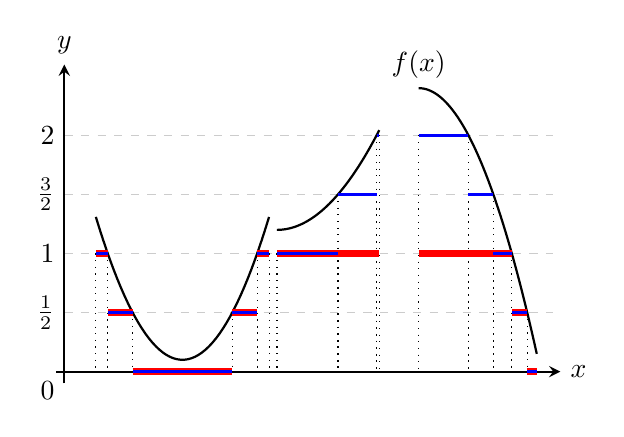
\begin{tikzpicture}[xscale=1, yscale=1.5, >=stealth]
                \foreach \y in {0.5, 1.0, 1.5, 2.0} {
                    \draw[gray!40, dashed, thin] (0,\y) -- (6.2,\y);
                }

                \draw[->, thick] (0,-0.1) -- (0,2.6) node[above] {$y$};
                \draw[->, thick] (-0.1,0) -- (6.3,0) node[right] {$x$};

                \node[below left] at (0,0) {$0$};
                \node[left] at (0, 0.5) {$\frac{1}{2}$};
                \node[left] at (0, 1.0) {$1$};
                \node[left] at (0, 1.5) {$\frac{3}{2}$};
                \node[left] at (0, 2.0) {$2$};

                \draw[thick, domain=0.4:2.6, samples=50] plot (\x, {(\x-1.5)^2 + 0.1});
                \draw[thick, domain=2.7:4.0, samples=50] plot (\x, {1.2 + 0.5*(\x-2.7)^2});
                \draw[thick, domain=4.5:6.0, samples=50] plot (\x, {2.4 - (\x-4.5)^2});

                \node[above] at (4.5, 2.4) {$f(x)$};

                \draw[black, dotted, thin] (0.4, 1.0) -- (0.4, 0);
                \draw[black, dotted, thin] (0.551, 1.0) -- (0.551, 0);
                \draw[black, dotted, thin] (0.551, 0.5) -- (0.551, 0);
                \draw[black, dotted, thin] (0.868, 0.5) -- (0.868, 0);
                \draw[black, dotted, thin] (2.132, 0.5) -- (2.132, 0);
                \draw[black, dotted, thin] (2.449, 0.5) -- (2.449, 0);
                \draw[black, dotted, thin] (2.449, 1.0) -- (2.449, 0);
                \draw[black, dotted, thin] (2.6, 1.0) -- (2.6, 0);

                \draw[black, dotted, thin] (2.7, 1.0) -- (2.7, 0);
                \draw[black, dotted, thin] (3.475, 1.0) -- (3.475, 0);
                \draw[black, dotted, thin] (3.475, 1.5) -- (3.475, 0);
                \draw[black, dotted, thin] (3.965, 1.5) -- (3.965, 0);
                \draw[black, dotted, thin] (3.965, 2.0) -- (3.965, 0);
                \draw[black, dotted, thin] (4.0, 2.0) -- (4.0, 0);

                \draw[black, dotted, thin] (4.5, 2.0) -- (4.5, 0);
                \draw[black, dotted, thin] (5.132, 2.0) -- (5.132, 0);
                \draw[black, dotted, thin] (5.132, 1.5) -- (5.132, 0);
                \draw[black, dotted, thin] (5.449, 1.5) -- (5.449, 0);
                \draw[black, dotted, thin] (5.449, 1.0) -- (5.449, 0);
                \draw[black, dotted, thin] (5.683, 1.0) -- (5.683, 0);
                \draw[black, dotted, thin] (5.683, 0.5) -- (5.683, 0);
                \draw[black, dotted, thin] (5.878, 0.5) -- (5.878, 0);
                \draw[black, dotted, thin] (5.878, 0) -- (5.878, 0);
                \draw[black, dotted, thin] (6.0, 0) -- (6.0, 0);

                \begin{scope}[red, line width=2.5pt]
                    \draw (0.4, 1.0) -- (0.551, 1.0);
                    \draw (0.551, 0.5) -- (0.868, 0.5);
                    \draw (0.868, 0) -- (2.132, 0);
                    \draw (2.132, 0.5) -- (2.449, 0.5);
                    \draw (2.449, 1.0) -- (2.6, 1.0);

                    \draw (2.7, 1.0) -- (4.0, 1.0);

                    \draw (4.5, 1.0) -- (5.683, 1.0);
                    \draw (5.683, 0.5) -- (5.878, 0.5);
                    \draw (5.878, 0) -- (6.0, 0);
                \end{scope}

                \begin{scope}[blue, line width=1.3pt]
                    \draw (0.4, 1.0) -- (0.551, 1.0);
                    \draw (0.551, 0.5) -- (0.868, 0.5);
                    \draw (0.868, 0) -- (2.132, 0);
                    \draw (2.132, 0.5) -- (2.449, 0.5);
                    \draw (2.449, 1.0) -- (2.6, 1.0);

                    \draw (2.7, 1.0) -- (3.475, 1.0);
                    \draw (3.475, 1.5) -- (3.965, 1.5);
                    \draw (3.965, 2.0) -- (4.0, 2.0);

                    \draw (4.5, 2.0) -- (5.132, 2.0);
                    \draw (5.132, 1.5) -- (5.449, 1.5);
                    \draw (5.449, 1.0) -- (5.683, 1.0);
                    \draw (5.683, 0.5) -- (5.878, 0.5);
                    \draw (5.878, 0) -- (6.0, 0);
                \end{scope}
            \end{tikzpicture}
            \vspace{-1cm}
        \end{center}
    \end{wrapfigure}

    We construct the sequence explicitly. Define \(s_1(x)=1\) wherever
    \(f(x)\geq1\), define \(s_1(x)=\frac12\) wherever
    \(\frac12\leq f(x)<1\), and define \(s_1(x)=0\) wherever
    \(f(x)<\frac12\). Denote these sets, respectively, by
    \begin{align*}
        E_0 &= f^{-1}([1,+\infty]),\\
        E_1 &= f^{-1}([\sfrac12,1)),\\
        E_\infty &= f^{-1}([0,\sfrac12)).
    \end{align*}

    To construct \(s_2\), divide \([0,2]\) into intervals of length
    \(\sfrac14\). Set \(s_2(x)=2\) when \(f(x)\geq2\), and assign to the
    remaining points the lower endpoint of the interval containing \(f(x)\).

    More generally, for every \(n\in\naturalnumbers^*\), divide \([0,n]\)
    into subintervals of length \(2^{-n}\), and set
    \begin{align*}
        E_{k,n}
        &=f^{-1}\!\left(\left[\frac{k}{2^n},\frac{k+1}{2^n}\right)\right),
        \qquad k=0,\ldots,n2^n-1,\\
        E_{\infty,n}&=f^{-1}([n,+\infty]).
    \end{align*}
    Since \(f\) is measurable, all these sets are measurable. Define
    \[
        s_n
        =\sum_{k=0}^{n2^n-1}\frac{k}{2^n}\indicator_{E_{k,n}}
        +n\indicator_{E_{\infty,n}}.
    \]
    Each \(s_n\) is therefore a nonnegative measurable simple function. The
    dyadic partitions refine as \(n\) increases, so
    \(s_n(x)\leq s_{n+1}(x)\leq f(x)\).

    If \(f(x)<+\infty\), then eventually
    \(0\leq f(x)-s_n(x)<2^{-n}\). If \(f(x)=+\infty\), then
    \(s_n(x)=n\to+\infty\). Hence \(s_n(x)\uparrow f(x)\) for every \(x\in X\).
    If \(f\) is bounded, choose \(M\) such that \(f\leq M\). For every \(n>M\),
    \(\lVert f-s_n\rVert_\infty\leq2^{-n}\), so the convergence is uniform.
    Conversely, if \(s_n\to f\) uniformly, choose \(N\) such that
    \(\lVert f-s_N\rVert_\infty<1\). Since \(s_N\) is bounded, \(f\) is bounded.
    \wrapfill
\end{snippetproof}

\begin{snippet}{riemann-lebesgue-partition-comparison}
    Riemann integration approximates a function by partitioning its domain.
    The construction above instead partitions the range into horizontal levels;
    this is the basic approximation underlying Lebesgue integration.
    Applying the construction to the positive and negative parts gives the
    corresponding approximation for real-valued measurable functions.
\end{snippet}

\end{document}
